
\section*{Overview}

There is a more general procedure we can use, in order to describe both DG-algebras and their model structure in one joint framework. The theory is developed in \cite{monoid} and uses so called monoids in monoidal categories. We will not cover all the details in this appendix, but we will go through the construction at least on a surface level. This is to get insight into how the theory presented in this thesis might be abstracted to other types of objects. 

Before we go into the theory, we give a brief overview of the process. Recall that DG-algebras are cochain complexes of vector spaces, with an added algebra structure, i.e. an associative product. This means that we can think of DG-algebras as a subcategory of $Ch(Vect_k)$, the category of cochain complexes of vector spaces over a field $k$. This category has two additional natural structures that we can add; a categorical product and a model structure. These extra structures are particularly nice in $Ch(Vect_k)$, which will allow us to transfer the model structure onto its subcategory of monoids. This subcategory will turn out to be the category of DG-algebras, $DGA_k$.

%The category of unbonded cochain complexes of vector spaces form a model category with weak equivalences being quasi-isomorphisms of cochain complexes, fibrations being degreewise surjections and cofibrations being the maps that satisfy the lifting property with respect to acyclic fibrations. This category is also a monoidal category, which means we have some form of product of object, in this case the tensor product of cochain complexes. This added monoidal structure plays nice with the model structure, so we get that the category of cochain complexes of vector spaces is a monoidal model category. The cofibrations and acyclic cofibrations turn out to have a generating set each, which we call being a cofibrantly generated model category. This means that we have a few extra tools we can use, most prominently the so-called small objects argument. 

%The category of DG-algebras is in fact the category of monoids in this monoidal model category. Since the underlying category is cofibrantly generated we can lift the model structure to its category of monoids, and hence we have a model structure (which coincides with the one we already described earlier) on the category of DG-algebras. 

\subsection*{Cofibrantly generated symmetric monoidal model categories}

The above chain of words is rather daunting, so lets build it up---step by step.

\begin{definition}[Monoidal category]
\index{Monoidal category}
A monoidal category is a category $\mathcal{C}$, equipped with a functor $\otimes : \mathcal{C} \times \mathcal{C} \rightarrow \mathcal{C}$, called the monoidal product, a unit object $1\in \mathcal{C}$ and three natural isomorphisms $\lambda_A : 1\otimes A \rightarrow A$, $\rho_A : A\otimes 1\rightarrow A$ and $\alpha_{A,B,C} : (A\otimes B)\otimes C \rightarrow A\otimes (B\otimes C)$ called the left unitor, right unitor and associator respectively---such that the following diagrams 

\begin{center}
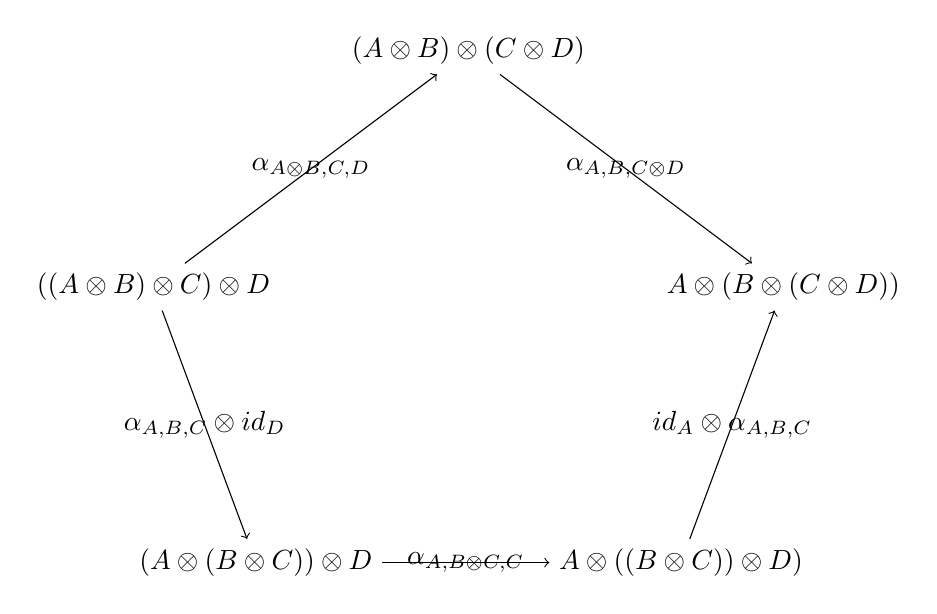
\begin{tikzpicture}
	\node (C) {};
	\node (1) [node distance=3cm, above of=C] {$(A\otimes B)\otimes (C\otimes D)$}; 
	\node (2) [node distance= 4cm, left of=C] {$((A\otimes B)\otimes C)\otimes D$};	
	\node (3) [node distance= 4cm, right of=C] {$A\otimes (B\otimes (C\otimes D))$};
	
	\node (D) [node distance=3.5cm, below of=C] {};
	\node (4) [node distance= 2.7cm, left of=D] {$(A\otimes (B\otimes C))\otimes D$};
	\node (5) [node distance= 2.7cm, right of=D] {$A\otimes ((B\otimes C))\otimes D)$};
	
	
	\draw [-to] (2) to node {$\alpha_{A\otimes B, C, D}$} (1);
	\draw [-to] (1) to node {$\alpha_{A, B, C\otimes D}$} (3);
	\draw [-to] (2) to node [swap]{$\alpha_{A, B, C}\otimes id_D$} (4);
	\draw [-to] (4) to node [swap]{$\alpha_{A, B\otimes C, C}$} (5);
	\draw [-to] (5) to node [swap]{$id_A\otimes \alpha_{A, B, C}$} (3);
\end{tikzpicture}
\end{center}

called the pentagon identity, and

\begin{center}
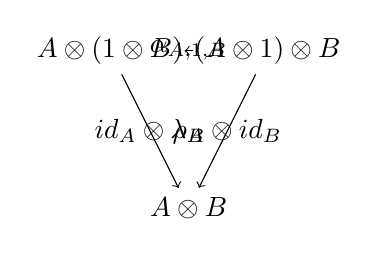
\begin{tikzpicture}
	\node (1) {$A\otimes (1\otimes B)$};
	\node (2) [right of=1] {};
	\node (3) [right of=2] {$(A\otimes 1)\otimes B$};
	\node (4) [node distance=2cm, below of=2] {$A\otimes B$};
	
	\draw [-to] (1) to node {$\alpha_{A, 1, B}$} (3);
	\draw [-to] (1) to node [swap]{$id_A\otimes \lambda_B$} (4);
	\draw [-to] (3) to node {$\rho_A\otimes id_B$} (4);
\end{tikzpicture}
\end{center}
called the triangle identity---both commute. 
\end{definition}

This definition can seem very abstract and difficult, but in reality it is quite simple. We are using the symbol for the tensor product, $\otimes $, for the monoidal product because the tensor product is usually the product we are using. So any intuition we have from using the tensor product can usually be applied to monoidal categories. If the three natural isomorphisms $ \lambda, \rho, \alpha $ are identities, then $ \mathcal{C}$ is called a strict monoidal category. These do rarely come up in nature, but every monoidal category is in fact equivalent to a strict monoidal category. Notice also $K4$ appearing as the pentagon identity. 

\begin{definition}[Symmetric monoidal category]
\index{Symmetric monoidal category}
Let $\mathcal{C}$ be a monoidal category. We say  $\mathcal{C}$ is a symmetric monoidal category if there is a natural isomorphism $\beta_{X,Y}: X\otimes Y \longrightarrow Y \otimes X$, called the braid isomorphism, such that $\beta_{X,Y}\circ \beta_{Y,X} = id_{X\otimes Y} $ and the following diagrams 
\begin{center}
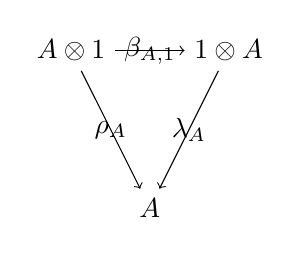
\begin{tikzpicture}
	\node (1) {$A\otimes 1$};
	\node (2) [right of=1] {};
	\node (3) [right of=2] {$1\otimes A$};
	\node (4) [node distance=2cm, below of=2] {$A$};
	
	\draw [-to] (1) to node {$\beta_{A, 1}$} (3);
	\draw [-to] (1) to node [swap]{$\rho_A$} (4);
	\draw [-to] (3) to node {$\lambda_A$} (4);
\end{tikzpicture}
\end{center}
called the unit coherence, and
\begin{center}
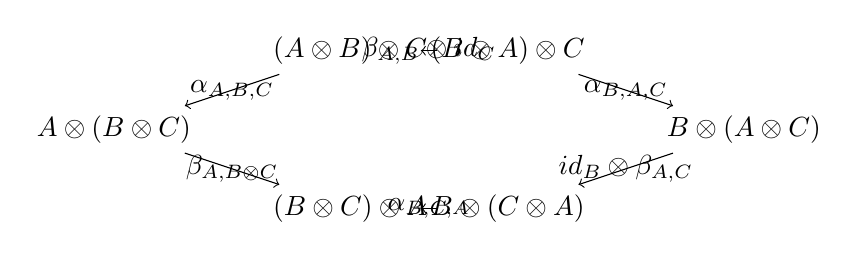
\begin{tikzpicture}
	\node (C) {};
	\node (1) [above of=C, left of=C] {$(A\otimes B)\otimes C$};
	\node (2) [above of=C, right of=C] {$(B\otimes A)\otimes C$};
	\node (3) [node distance=4cm, left of=C] {$A\otimes(B\otimes C)$};
	\node (4) [node distance=4cm, right of=C] {$B\otimes (A\otimes C)$};
	\node (5) [below of=C, left of=C] {$(B\otimes C)\otimes A$};
	\node (6) [below of=C, right of=C] {$B\otimes (C\otimes A)$};
	
	\draw [-to] (1) to node {$\beta_{A, B}\otimes id_C$} (2);
	\draw [-to] (1) to node [swap]{$\alpha_{A, B, C}$} (3);
	\draw [-to] (2) to node {$\alpha_{B, A, C}$} (4);
	\draw [-to] (3) to node [swap]{$\beta_{A, B\otimes C}$} (5);
	\draw [-to] (5) to node [swap]{$\alpha_{B, C, A}$} (6);
	\draw [-to] (4) to node {$id_B\otimes \beta_{A, C}$} (6);
\end{tikzpicture}
\end{center}
called the associativity coherence, both commute. 
\end{definition}

A monoidal category can be thought of as a category with a multiplication, an a symmetric monoidal category is then a monoidal category with a commutative product. 

\begin{definition}[Closed symmetric monoidal category]
\index{Closed symmetric monoidal category}
Let $\C$ be a symmetric monoidal category. We say $\C$ is closed if the tensor functor $-\otimes A\colon \C \longrightarrow \C$ has a right adjoint functor $[A, -]\colon \C \longrightarrow \C$, called the internal hom. 
\end{definition}

The notion of closed category can be defined without the need for a symmetric monoidal structure, but this definition is a bit more involved---and the above definition is the result of combining the closed structure with the symmetric monoidal one. 

We can think about this as being motivated by---or at least inspired by the category of sets---where we have $[X,Y]=\{ f:X\longrightarrow Y\}$, and $Hom(S, [X, Y])\cong Hom(S\times X, Y)$. So when we require that the internal hom functor $[A,-]$ is a right adjoint to the monoidal product functor $-\otimes A$, we get a bijection $Hom(X, [A, B])\longrightarrow Hom(X\otimes A, B)$, that is natural in all three variables. This isomorphism is called ``currying''.

\begin{definition}[Pushout product]
\index{Pushout product}
Let $\C$ be a symmetric monoidal category and $f\colon A\longrightarrow B$, $f'\colon A'\longrightarrow B'$ be morphisms in $\C$. We can form the following pushout diagram
\begin{center}
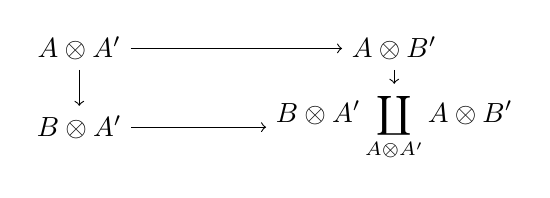
\begin{tikzpicture}
	\node (1) {$A\otimes A'$};
	\node (3) [below of=1] {$B\otimes A'$};
	\node (2) [node distance=4cm, right of=1] {$A\otimes B'$};
	\node (4) [below of=2] {${\displaystyle B\otimes A'\coprod_{A\otimes A'}A\otimes B'}$};

	\draw [-to] (1) to node {} (2);
	\draw [-to] (1) to node {} (3);
	\draw [-to] (2) to node {} (4);
	\draw [-to] (3) to node {} (4);	
\end{tikzpicture}
\end{center}
By the universal property of pushouts we get an induced map
\begin{equation*}
    B\otimes A' \coprod_{A\otimes A'} A\otimes B' \longrightarrow B\otimes B'
\end{equation*}
which we call the pushout product of $f$ and $f'$. 
\end{definition}

We have already covered the definition of a model category\index{Model category} in the thesis, so recall that it consists of three classes of maps $W, C, F$---called weak equivalences\index{Weak equivalence}, cofibrations\index{Cofibration} and fibrations\index{Fibration} respectively---such that certain axioms \textbf{MC1}, \textbf{MC2}, \textbf{MC3} and \textbf{MC4} hold. 

\begin{definition}[Symmetric monoidal model category]\index{Symmetric monoidal model category}
A (closed) symmetric monoidal model category is a category $\C$ with a model structure $(W, C, F)$, equipped with the structure of a closed symmetric monoidal category $(\otimes, I)$, such that the pushout product of two cofibrations is again a cofibration, the pushout product of a cofibration and an acyclic cofibration is again an acyclic cofibration and that the map $QI\otimes X \overset{p\otimes id_X}\longrightarrow I\otimes X \longrightarrow X$ between any cofibrant object $X$---and any cofibrant replacement $QI$ of the tensor unit $I$---is a weak equivalence. 
\end{definition}

We are almost at the end, but we need one more ``niceness'' condition on our category $\C$. We now have that the monoidal structure is nice, and respects the model structure, but we also want the model structure itself to be ``nice''. The rigorous definition of this niceness condition is a bit tricky, but it essentially requires the cofibrations and the acyclic cofibrations to be generated by a small set. 

If we let $P$ be some set of morphisms in $\C$ then let 
\begin{itemize}
    \item $P-inj$ be the morphisms in $\C$ that satisfy the right lifting property with respect to the morphisms in $P$. These are called the $P$-injectives.
    \item $P-cof$ be the morphisms that satisfy the left lifting property with respect to $P-inj$. These are called the $P$-cofibrations
    \item $P-reg \subseteq P-cof$ the maps in $\C$ that are transfinite conpositions of pushouts of morphisms in $P$. These morphisms are called the regular $P$-cofibrations. 
\end{itemize}

\begin{definition}[Cofibrantly generated model category]
\index{Cofibrantly generated model category}
Let $\C$ be a category with a model structure $(W, C, F)$. We say $\C$ is cofibrantly generated if there are subsets $P\subseteq C$ and $Q\subseteq C\cap W$ such that 
\begin{itemize}
    \item $F = Q-inj$
    \item $C\cap W = P-inj$
    \item $C = P-cof$
    \item $C\cap W = Q-cof$ 
    \item The domain of a morphism in $P$ is a small relative of $P-reg$
    \item The domain of a morphism in $Q$ is a small relative of $Q-reg$
\end{itemize}
\end{definition}

We have not defined the last two points in the definition above. We wont cover these in detail, as they are complicated and not necessary for the surface overview that we are presenting. It essentially means that $Hom(C,-)$---for an object $C$, that is the domain of a map in $P$ or $Q$---commutes with colimits in $P-reg$ or $Q-reg$ respectively. For the details see \cite{monoid}. 

We then have the category we want, i.e. $\C$ a cofibrantly generated closed symmetric monoidal model category. The next task is to find the correct subcategory. 





\subsection*{The category of monoids}

\begin{definition}[Monoid in a monoidal category]
\index{Monoid in a monoidal category}
A monoid in a monoidal category $ (\mathcal{C}, \otimes, I)$ is an object $ M$ together with a map $ \mu:M\otimes M\longrightarrow M$, called multiplication, and a map $ \eta: I\longrightarrow M$, called the unit, such that the associative law and left and right unit laws hold, i.e. the following three diagrams commute
\begin{center}
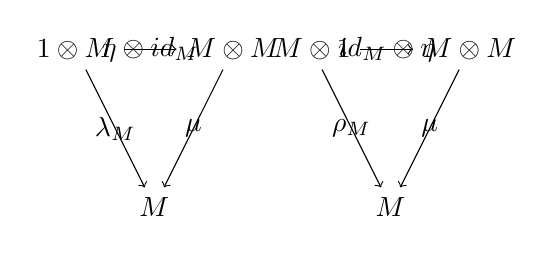
\begin{tikzpicture}
	\node (1) {$1\otimes M$};
	\node (2) [right of=1] {};
	\node (3) [right of=2] {$M\otimes M$};
	\node (4) [node distance=2cm, below of=2] {$M$};
	
	\node (5) [right of=3] {$M\otimes 1$};
	\node (6) [right of=5] {};
	\node (7) [right of=6] {$M\otimes M$};
	\node (8) [node distance=2cm, below of=6] {$M$};	
	
	\draw [-to] (1) to node {$\eta\otimes id_M$} (3);
	\draw [-to] (1) to node [swap]{$\lambda_M$} (4);
	\draw [-to] (3) to node {$\mu$} (4);
	
	\draw [-to] (5) to node {$id_M\otimes \eta$} (7);
	\draw [-to] (5) to node [swap]{$\rho_M$} (8);
	\draw [-to] (7) to node {$\mu$} (8);	
\end{tikzpicture}
\end{center}

\begin{center}
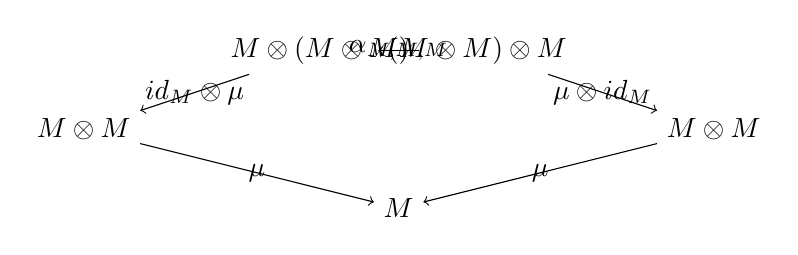
\begin{tikzpicture}
	\node (C) {};
	\node (1) [above of=C, left of=C] {$M\otimes (M\otimes M)$};
	\node (2) [above of=C, right of=C] {$(M\otimes M)\otimes M$};
	\node (3) [node distance=4cm, left of=C] {$M\otimes M$};
	\node (4) [node distance=4cm, right of=C] {$M\otimes M$};
	\node (5) [below of=C] {$M$};


	\draw [-to] (1) to node {$\alpha_{M, M, M}$} (2);
	\draw [-to] (1) to node [swap]{$id_M\otimes \mu$} (3);
	\draw [-to] (2) to node {$\mu\otimes id_M$} (4);
	\draw [-to] (3) to node [swap]{$\mu$} (5);
	\draw [-to] (4) to node {$\mu$} (5);	

\end{tikzpicture}
\end{center}
\end{definition}

Here $ \alpha$ is the associator in the monoidal category and $ \lambda, \rho$ are the unitors. We see that this notion of monoid in a monoidal category produces the standard notion of a monoid from algebra---if we let the monoidal category be $Set$ together with the cartesian product. 

The collection of monoids in a monoidal category $\C$ do in fact form a category themselves, which we denote by $Mon\C$. The following theorem is \cite[Theorem 4.1 (3)]{monoid}, and it assures us that we get a model structure on the category of monoids.

\begin{theorem}
Let $\C$ be a cofibrantly generated symmetric monoidal model category. If $R$ is a commutative monoid in $\C$, then the category of $R$-algebras is a cofibrantly generated model category. 
\end{theorem}

If we let $R$ be the monoidal unit $I$ in the theorem above, we have $I$-mod = $Mon\C$, meaning we have a model structure on the category of monoids. This model structure is induced from the one in $\C$, meaning that a morphism in $Mon\C$ is a fibration or a weak equivalence if it is a fibration or a weak equivalence in $\C$, and that the cofibrations in $Mon\C$ are the ones having the left lifting property with respect to the acyclic fibrations. 

\subsection*{Model structure on $DGA_k$}

We have now laid out the general machinery, so what's left is to apply it to our situation. We start with $Ch(Vect_k)$, the category of cochain complexes of vector spaces over a field $k$. It has a symmetric monoidal product given by the graded tensor product, i.e.
\begin{equation*}
    (A\otimes B)^n = \sum_{i+j=n} A^i \otimes B^j , 
\end{equation*}
which has differential given by $d_{A\otimes B} = d_A\otimes id_A + id_B\otimes d_B$. 

As we have used throughout the thesis, we know that morphisms $Hom(A, B)$ also form cohain complexes, hence we have an internal hom. We have a model structure, given by degreewise surjections being the fibrations, the weak equivalences being the quasi-isomorphisms and the cofibrations being the maps that have the left lifting property with respect to acyclic fibrations. In \cite[Theorem 2.3.11]{hovey} it is proven that this model structure makes $Ch(Vect_k)$ into a cofibrantly generated model category. 

Hence we have the following theorem to summarize the informal discussion. 

\begin{theorem}
The category $Ch(Vect_k)$ is a cofibrantly generated symmetric monoidal model category.
\end{theorem}

The last piece of the puzzle is showing that the monoids in $Ch(Vect_k)$ are in face the DG-algebras. 

A monoid in $Ch(Vect_k)$ is an object $A$, together with a map $m\colon A\otimes A\longrightarrow A$, and a map $\eta\colon k\longrightarrow A$, such that the left and right unit laws, and the associative law hold. This means that we have a cochain complex of vector spaces together with an associative multiplication map, $m$. 

The fact that $m$ is a morphism of cochain complexes means that we have a commutative diagram
\begin{center}
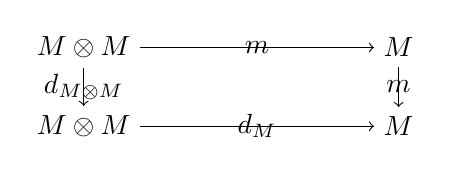
\begin{tikzpicture}
	\node (1) {$M\otimes M$};
	\node (3) [below of=1] {$M\otimes M$};
	\node (2) [node distance=4cm, right of=1] {$M$};
	\node (4) [below of=2] {$M$};

	\draw [-to] (1) to node {$m$} (2);
	\draw [-to] (1) to node [swap]{$d_{M\otimes M}$} (3);
	\draw [-to] (2) to node {$m$} (4);
	\draw [-to] (3) to node [swap]{$d_M$} (4);	
\end{tikzpicture}
\end{center}
And hence that
\begin{align*}
    d_M\circ m
    &= m\circ d_{M\otimes M} \\
    &= m(d_M\otimes id_M) + m(id_M\otimes d_M)
\end{align*}
which gives 
\begin{equation*}
    d_M(m(a\otimes b) = m(d_M(a)\otimes b) + (-1)^{|a|}m(a\otimes d_M(b))
\end{equation*}
when applied to elements and using the Koszul grading rule\index{The Koszul grading rule}. If we write $m(a\otimes b) = a\cdot b$ then we get the familiar graded Leibniz rule\index{The Leibniz rule} 
\begin{equation*}
    d_M(a\cdot b) = d_M(a)\cdot b + (-1)^{|a|}a\cdot d_M(b).
\end{equation*}

Thus, a monoid in $Ch(Vect_k)$ is in fact a DG-algebra\index{DG-algebra}. We then get an induced model structure on $Mon(Ch(Vect_k)) = DGA_k$, which we can identify with Jardine's model structure we constructed earlier in the thesis.

